\section{Introduction}
Analysis of RADAR systems in maritime environments is complicated by the fact that the ocean does not generally provide a smooth or uniform surface to work with. Altitude variations change the aspect angle for multipath bounces, induce wave blockage, and add clutter and spikes to the echo return \cite{skolnik_handbook}, \cite{blake_radar}, \cite{nathanson_radar}. These are random effects which induce signal fluctuations that have a significant impact on the probability of detecting a target. Understanding the impact of the sea surface on propagation is critical to evaluating the performance of a RADAR system in a maritime environment.

When we look at cases where the transmitter and receiver are not colocated, we have a bistatic configuration and analyzing performance becomes even more difficult \cite{willis_bistatic}. We cannot leverate reciprocity as the paths are no longer constant, and the effects of multipath and clutter are often skewed due to geometric differences.  In addition, the receiver observes the target from a different aspect angle than it was illuminated with, resulting in a different radiation pattern. With multiple receivers or transmitters, the configuration is termed multistatic as there are multiple bistatic elements.

\subsection{Objective}
The primary objective of this work is to evaluate the performance of multistatic Radio Frequency (RF) sensor networks through 2 aims: 1) demonstrate that Random Matrix Theory (RMT) allows prediction of the signal statistics; and 2) investigate contributions from multipath and clutter to characterize potential engagement geometries. 

Aim 1 will be accomplished in three phases. First, the ocean surface will be modeled to ensure that the appropriate sea wave statistics are captured in both the down range and cross range directions. Second, a Monte Carlo study will be performed to generate signal statistics. This study will be executed by generating a series of sea surfaces and then numerically propagating a signal through a Parabolic Wave Equation (PWE) solver. Finally, RMT will be used to generate a statistical model that encompasses the results.

Aim 2 will be accomplished in two phases. First, bistatic clutter will be investigated to understand its impacts. Second, the results of Aim 1 will be folded in to understand how interference effects from clutter and multipath evolve through various engagement geometries.

\subsection{Multistatic RF Sensor Network Concept}
An example multistatic RF sensor network in a maritime environment is shown in Figure \ref{ms_fig:1}. In this concept, a single transmitter illuminates a target and the echo signal is captured by a pair of receivers. The received signal will fluctuate due to multipath reflections from the surface and relative motion of the target.

\begin{figure}[H]
  \begin{center}
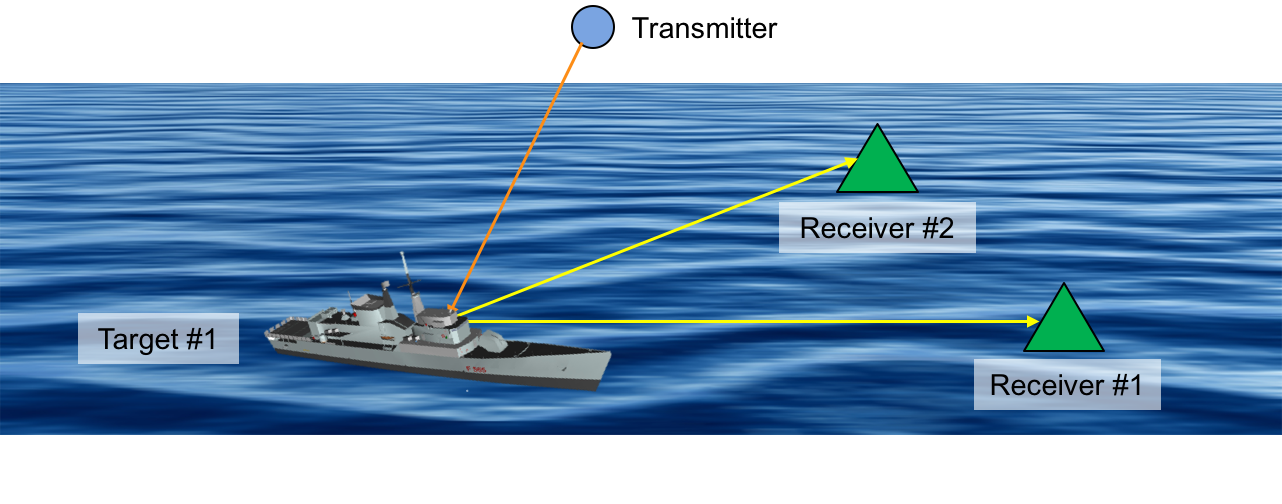
\includegraphics[width=5in]{../media/multistatic/ms_rf_concept.png}
  \end{center}
  \renewcommand{\baselinestretch}{1} \small\normalsize
  \begin{quote}
    \caption[Multistatic RF Sensor Networks Concept]{Multistatic RF Sensor Networks Concept\label{ms_fig:1}}
  \end{quote}
\end{figure}
\renewcommand{\baselinestretch}{2} \small\normalsize

\subsubsection{Sources of Uncertainty}
There are 3 primary sources for randomness in propagating through a maritime environment: 1) the configuration of the target ship; 2) the refractivity of the atmosphere; and 3) the sea surface.

The configuration of the target ship drives the RADAR Cross Section (RCS). As shown in Figure \ref{rmt_fig:1}, the RCS signature is complicated and highly aspect dependent. 

\begin{figure}[H]
  \begin{center}
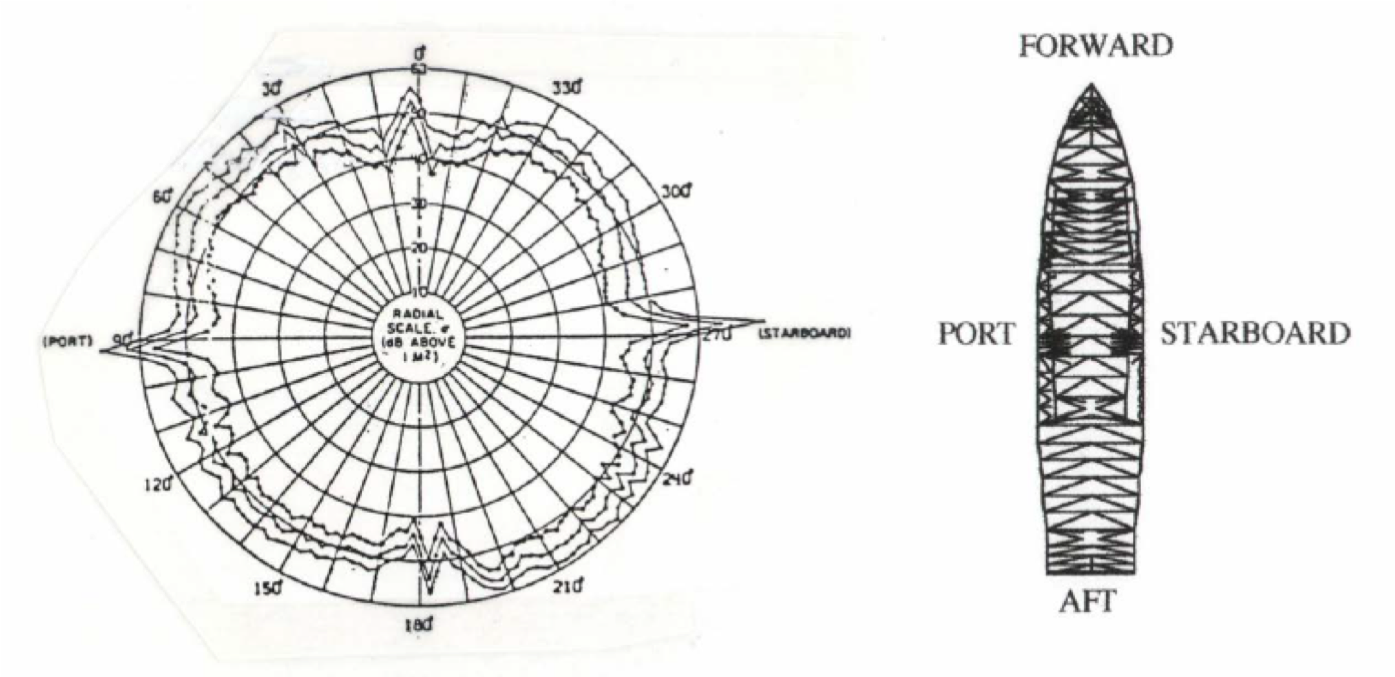
\includegraphics[width=4.5in]{../media/multistatic/shipconfig.png}
  \end{center}
  \renewcommand{\baselinestretch}{1} \small\normalsize
  \begin{quote}
    \caption[Ship Configuration RCS]{Ship Configuration RCS\label{rmt_fig:1}}
  \end{quote}
\end{figure}
\renewcommand{\baselinestretch}{2} \small\normalsize

The RCS is also impacted by how the specific ship is configured; what it has or doesn't have and how components are arranged on the deck. There are many research programs applying significant effort into modeling the behavior of ship RCS signatures, so RCS fluctuations will be considered out of scope for the purposes of this work.

The next source of uncertainty is the refractive index profile of the atmosphere, which can vary significantly as described in Chapter \ref{chapter_env}. As shown in Figure \ref{rmt_fig:2}, a transmitted ray will refract in the atmosphere and follow a curved path. With standard atmospheric conditions, the refractivity gradient is negative and the rays bend towards the earth. As the gradient becomes more negative (due to temperature, humidity, pressure, etc.), the rays curve more strongly towards the earth. At a critical point when the radius of curvature of a ray equals the radius of curvature of the earth, the atmosphere acts as a wave guide and effectively traps the rays. This last condition is known as a duct.

\begin{figure}[H]
  \begin{center}
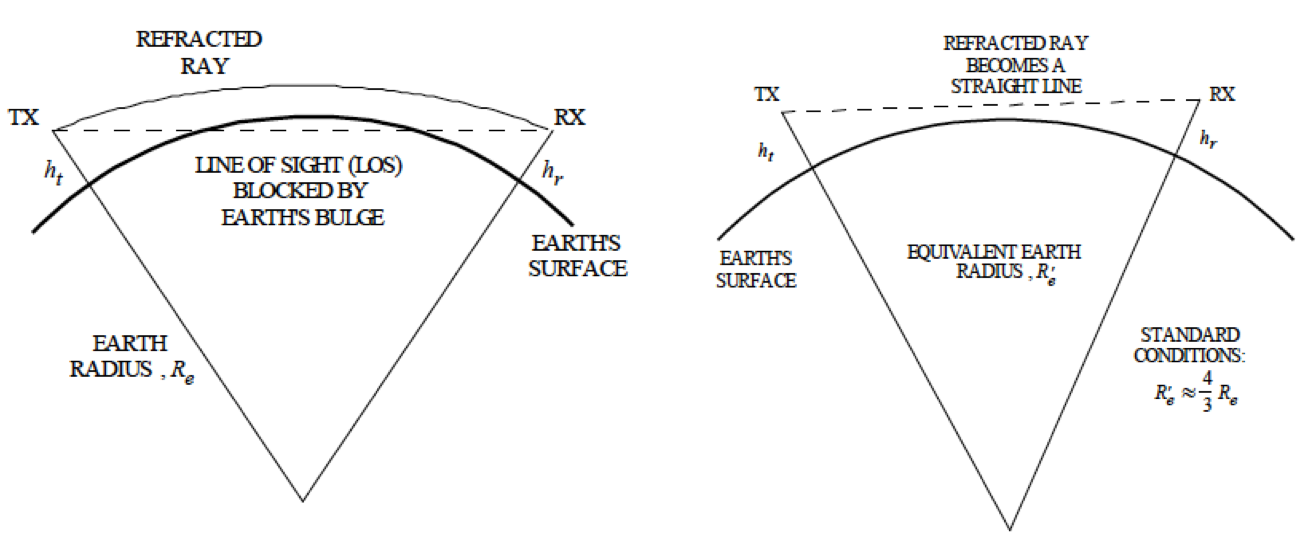
\includegraphics[width=6in]{../media/multistatic/earth_refractivity.png}
  \end{center}
  \renewcommand{\baselinestretch}{1} \small\normalsize
  \begin{quote}
    \caption[Atmospheric Refractivity Profiles]{Atmospheric Refractivity Profiles\label{rmt_fig:2}}
  \end{quote}
\end{figure}
\renewcommand{\baselinestretch}{2} \small\normalsize

Large scale variations in refractivity occur on the order of several minutes to hours and will not significantly impact the signal statistics over a few pulses or a Coherent Processing Interval (CPI). We will treat refractive index fluctuations as affecting average signal levels rather than variance.

The final source of uncertainty is variations due to the sea surface, which manifest through multipath and clutter. Multipath is due to interference from forward scattering and clutter is due to backscatter from the surface. Propagation through a duct will have higher signal variation than propagation without a duct, especially at longer ranges. This is because the rays in a duct will reflect from the surface multiple times while rays outside of a duct will only have a single reflection from the surface.
